\section{Requirements}
This section outlines the functional requirements of the F-LOW Food Delivery Service system. It includes the main use case diagram showing the fundamental interactions among users and the system, followed by detailed descriptions of each use case scenario. These requirements form the basis for understanding system functionality and are essential inputs for the subsequent architectural design using the 4+1 view model.

\subsection{Use case diagram}

\begin{figure}[htbp]
  \centering
  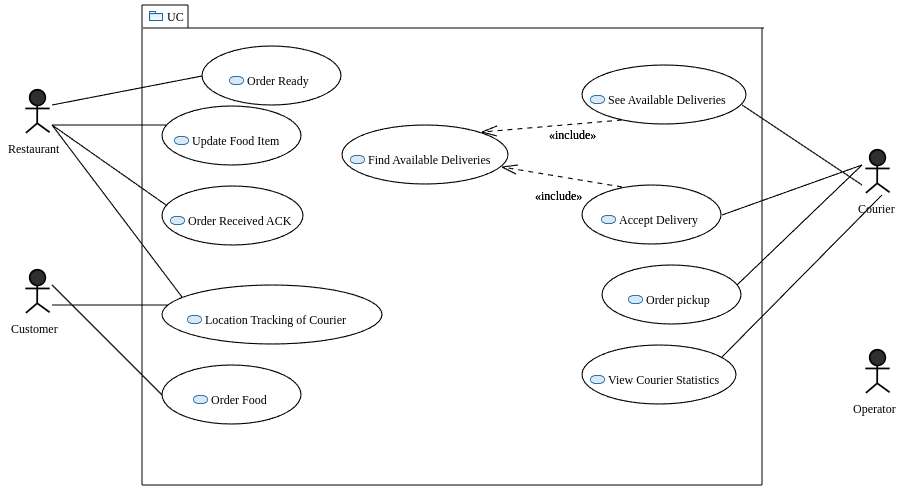
\includegraphics[width=0.8\textwidth]{FIGS/UCD-Apr6-v1.png}  % change filename and width as needed
  \caption{Use Case Diagram. This diagram comprises four actors, nine base use cases, and one inclusion use case.}
  \label{fig:my_label}
\end{figure}

\subsection{Use cases description}

\subsubsection{Updating food item menu}

\noindent
\begin{tabularx}{\textwidth}{l X}
    \textbf{Identifier and Name} & UC-1: Updating food item menu \\
    \textbf{Actors} & Restaurant \\
    \textbf{Preconditions} & 
    \begin{itemize} 
        \item The restaurant is logged into the system  
        \item The restaurant has permission to modify its menu
    \end{itemize} \\
    \textbf{Main Success Scenario} & The restaurant accesses the menu update section and enters the updated information for a given food item. Then the system validates the changes (Exn 1.) made by the restaurant and the menu gets updated. \\
    \textbf{Exceptions} & \begin{itemize} 
        \item \textbf{Exn 1.} Invalid food item details 
         \begin{itemize} 
            \item The restaurant gives information the system can not process.
            \item The system displays an error message and requests for changes.
         \end{itemize}
    \end{itemize} \\
    \textbf{Expected Result} & The restaurant's menu is updated and users can now order it. 
\end{tabularx}


\subsubsection{Order Received Acknowledgement}

\noindent
\begin{tabularx}{\textwidth}{l X}
    \textbf{Identifier and Name} & UC-2: Order Received Acknowledgement \\
    \textbf{Actors} & Restaurant, Customer \\
    \textbf{Preconditions} & 
    \begin{itemize} 
        \item A customer has placed an order in the system.  
        \item The restaurant has successfully received an order request.
    \end{itemize} \\
    \textbf{Main Success Scenario} & The system notifies the restaurant about the new order request (Exn 1.). Then the restaurant reviews the order details  and acknowledges it (Exn 2.), making the system send a notification to the user which is displayed in the UI. \\
    \textbf{Exceptions} & \begin{itemize} 
        \item \textbf{Exn 1.} Restaurant's system is down
         \begin{itemize} 
            \item The restaurant's system is disconnected or down so order requests can not come in.
            \item The system retries for some time with the request.
            \item The system notifies about the issue to customer support team and the user.
         \end{itemize}
         \item \textbf{Exn 2.} Restaurant declines order
         \begin{itemize} 
            \item The restaurant declines an order due to overload.
            \item The system tells the user about the issue.
         \end{itemize}
    \end{itemize} \\
    \textbf{Expected Result} & The restaurant starts working on the new order and the user is assured about it.
\end{tabularx}

\subsubsection{Order Ready for Delivery}

\noindent
\begin{tabularx}{\textwidth}{l X}
    \textbf{Identifier and Name} & UC-3: Order Ready for Delivery \\
    \textbf{Actors} & Restaurant, Customer, Courier \\
    \textbf{Preconditions} & 
    \begin{itemize} 
        \item A customer has placed an order in the system.  
        \item The restaurant has successfully received and processed an order request.
        \item A courier has accepted the delivery from the restaurant.
    \end{itemize} \\
    \textbf{Main Success Scenario} & The restaurant marks as ready for delivery the processed order. The system then notifies the courier who accepted the delivery for pickup. The user is also notified that the order is ready. \\
    \textbf{Exceptions} & \begin{itemize} 
        \item \textbf{Exn 1.} Delay in processing the order
         \begin{itemize} 
            \item The restaurant can not prepare the order in the estimated time.
            \item The system allows the restaurant to update the estimated time for delivery.
            \item The system updates the estimated time and notifies the user.
         \end{itemize}
    \end{itemize} \\
    \textbf{Expected Result} & The courier receives a notification about the order being ready for pickup and the customer as well.
\end{tabularx}

\subsubsection{Food Ordering}

\noindent
\begin{tabularx}{\textwidth}{l X}
    \textbf{Identifier and Name} & UC-4: Food Ordering \\
    \textbf{Actors} & Customer \\
    \textbf{Preconditions} & 
    \begin{itemize} 
        \item The customer is logged into the system.
        \item The restaurant menu is available for viewing and ordering.
    \end{itemize} \\
    \textbf{Main Success Scenario} & The customer begins by browsing the available food items on the menu. Once the customer selects the desired items, the system displays them with their respective prices and the total cost of the order. The customer then proceeds to the checkout, where they enter their payment details. The system processes the payment and confirms the order, showing a summary of the items ordered and an estimated delivery time. The customer receives a confirmation notification with the expected time of arrival. \\
    \textbf{Exceptions} & \begin{itemize} 
        \item \bold{ \textbf{Exn 1.} Invalid Payment:} If the payment method is declined, the system will display an error message and prompt the customer to enter a different payment method.
        \item \bold{ \textbf{ Exn 2.} Out of Stock Items:} If any of the selected items are unavailable, the system will notify the customer and offer them the option to modify their order, such as selecting alternative items.
    \end{itemize} \\
    \textbf{Expected Result} & The customer’s order is successfully placed, and the restaurant begins preparing the food. The customer receives notifications about the status of the order, including the estimated delivery time.
\end{tabularx}

\subsubsection{Location Tracking of Courier}

\noindent
\begin{tabularx}{\textwidth}{l X}
    \textbf{Identifier and Name} & UC-5: Location Tracking of Courier \\
    \textbf{Actors} & Customer, Restaurant \\
    \textbf{Preconditions} & 
    \begin{itemize} 
        \item The courier has accepted the delivery and is en route to the customer.
        \item The customer is logged into the system and has placed an order.
    \end{itemize} \\
    \textbf{Main Success Scenario} & Once the courier has accepted the delivery, the system begins tracking their location in real-time. The customer is able to see the courier’s current location on the app, and the system continuously updates the customer with notifications, including the courier’s progress and the estimated time of arrival. As the courier approaches the destination, the customer receives a notification indicating that the order will be delivered shortly. The customer is kept informed of any status changes until the order is successfully delivered. \\
    \textbf{Exceptions} & \begin{itemize} 
        \item \bold{ \textbf{Exn 1.} Courier’s GPS Signal Lost:} If the courier’s GPS signal is lost, the system will notify the customer about the temporary delay in tracking and will update the customer once the signal is restored.
        \item \bold{ \textbf{Exn 2.} Courier Delayed:} If the courier experiences a delay due to traffic or other unforeseen issues, the system will update the customer with a revised estimated arrival time.
    \end{itemize} \\
    \textbf{Expected Result} & The customer can track the courier’s real-time location throughout the delivery process and receive notifications until the order is delivered successfully.
\end{tabularx}

\subsubsection{See Available Deliveries}

\noindent
\begin{tabularx}{\textwidth}{l X}
    \textbf{Identifier and Name} & UC-6: See Available Deliveries \\
    \textbf{Actors} & Courier \\
    \textbf{Preconditions} & 
    \begin{itemize} 
        \item The courier is logged into the mobile app.
        \item Location permissions are granted.
        \item The courier is marked as available for deliveries.
    \end{itemize} \\
    \textbf{Main Success Scenario} & INCLUDE(UC-I-1). Each delivery displays relevant information such as the restaurant name, destination area, estimated distance, and compensation. \\
    \textbf{Exceptions} & 
    \begin{itemize} 
        \item \textbf{Exn 1.} No active deliveries in the area
        \begin{itemize}
            \item The app displays a message indicating no deliveries are currently available and may suggest checking again later.
        \end{itemize}
        \item \textbf{Exn 2.} GPS unavailable
        \begin{itemize}
            \item The app displays an error and requests permission to enable location services or suggests troubleshooting.
        \end{itemize}
    \end{itemize} \\
    \textbf{Expected Result} & The courier sees an updated list of deliveries that they are eligible to accept based on their current location and availability.
\end{tabularx}

\subsubsection{Accept Delivery}

\noindent
\begin{tabularx}{\textwidth}{l X}
    \textbf{Identifier and Name} & UC-7: Accept Delivery \\
    \textbf{Actors} & Courier \\
    \textbf{Preconditions} & 
    \begin{itemize} 
        \item The courier is logged into the mobile app.
        \item The courier has viewed the list of available deliveries.
        \item The courier does not currently have an active delivery in progress.
    \end{itemize} \\
    \textbf{Main Success Scenario} & INCLUDE(UC-I-1). The courier selects a delivery from the list and taps “Accept.” The system checks the availability in real-time. If still available, the system reserves the order for the courier, updates the order state, and notifies the restaurant that a courier has accepted the delivery. A confirmation is shown to the courier. \\
    \textbf{Exceptions} & 
    \begin{itemize} 
        \item \textbf{Exn 1.} Delivery already accepted by another courier
        \begin{itemize}
            \item The system informs the courier that the delivery is no longer available and prompts them to refresh the list.
        \end{itemize}
        \item \textbf{Exn 2.} Network failure
        \begin{itemize}
            \item The system retries the request a few times. If it still fails, an error message is shown to the courier.
        \end{itemize}
    \end{itemize} \\
    \textbf{Expected Result} & The delivery is now assigned to the courier. The app transitions to the next step in the delivery workflow (i.e., pickup).
\end{tabularx}


\subsubsection{Order Pickup}

\noindent
\begin{tabularx}{\textwidth}{l X}
    \textbf{Identifier and Name} & UC-8: Order Pickup \\
    \textbf{Actors} & Courier \\
    \textbf{Preconditions} & 
    \begin{itemize} 
        \item The courier is logged into the mobile app.
        \item the courier has already accepted the order and the delivery is assigned to them.
    \end{itemize} \\
    \textbf{Main Success Scenario} & The courier initially picks up the order from the restaurant. Afterward, they will change the status of delivery to "Picked Up" (Exn 1). \\
    \textbf{Exceptions} & 
    \begin{itemize} 
        \item \textbf{Exn 1.} Order already picked up by courier
        \begin{itemize}
            \item The system informs the courier that the status of the delivery has already been changed to "Pick Up" by the courier.
        \end{itemize}
    \end{itemize} \\
    \textbf{Expected Result} & The delivery is now picked up by the courier. The app transitions to the next step in the delivery workflow (i.e., deliver).
\end{tabularx}

\subsubsection{View Courier Statistics}

\noindent
\begin{tabularx}{\textwidth}{l X}
    \textbf{Identifier and Name} & UC-9: View Courier Statistics \\
    \textbf{Actors} & Courier \\
    \textbf{Preconditions} & 
    \begin{itemize} 
        \item The courier is logged into the mobile app.
    \end{itemize} \\
    \textbf{Main Success Scenario} & The courier navigates to the statistics section of the UI. The system asks for the start date and the end date of the period for which the courier wants the statistics (Exn 1). \\
    \textbf{Exceptions} & 
    \begin{itemize} 
        \item \textbf{Exn 1.} Order already picked up by courier
        \begin{itemize}
            \item The system informs the courier that the status of the delivery has already been changed to "Pick Up" by the courier.
        \end{itemize}
    \end{itemize} \\
    \textbf{Expected Result} & The delivery is now picked up by the courier. The app transitions to the next step in the delivery workflow (i.e., deliver).
\end{tabularx}

\subsubsection{Order Payment}

\noindent

\subsubsection{Order Delayed}

\noindent
\begin{tabularx}{\textwidth}{l X}
    \textbf{Identifier and Name} & UC-11: Order Delayed \\
    \textbf{Actors} & Courier \\
    \textbf{Preconditions} & 
    \begin{itemize} 
        \item The courier has started a delivery.
    \end{itemize} \\
    \textbf{Main Success Scenario} & The courier accesses the interface where they update the time of delivery. \\
    \textbf{Exceptions} & \\
    \textbf{Expected Result} & The system updates the information about delivery time to the customer.
\end{tabularx}

\subsubsection{Delivery completed}

\noindent
\begin{tabularx}{\textwidth}{l X}
    \textbf{Identifier and Name} & UC-12: Delivery completed \\
    \textbf{Actors} & Courier \\
    \textbf{Preconditions} & 
    \begin{itemize} 
        \item The courier has started a delivery.
    \end{itemize} \\
    \textbf{Main Success Scenario} & The courier accesses the interface and sets the delivery as completed. \\
    \textbf{Exceptions} & \\
    \textbf{Expected Result} & The customer can see its delivery in the completed state as well as the courier.
\end{tabularx}


\subsection{Inclusion Use Cases}

\subsubsection{Find Available Deliveries}

\noindent
\begin{tabularx}{\textwidth}{l X}
    \textbf{Identifier and Name} & UC-I-1: Find Available Deliveries \\
    \textbf{Actors} & Courier \\
    \textbf{Preconditions} & 
    \begin{itemize} 
        \item The courier is logged into the mobile app.
    \end{itemize} \\
    \textbf{Main Success Scenario} & The courier opens the app and navigates to the “Available Deliveries” section. The system fetches a list of current delivery orders in the area that have not yet been accepted. \\
    \textbf{Exceptions} & 
     - \\
    \textbf{Expected Result} & The system displays to the courier a list of current delivery orders in the area that have not yet been accepted.
\end{tabularx}